%% Q1 ctx
\textbf{Q.~1--5:} The table below shows the number of students admitted to different colleges I, II, III, IV and V in a particular session in various disciplines. Refer to the table to answer the questions 1--5 that follow.
\begin{center}\small
\begin{tabular}{lccccc|c}\toprule \textbf{Discipline} & MBA & B.Tech & B.Sc. & B.Com. & B.A. & \\
\textbf{Capacity} & 200 & 200 & 400 & 300 & 500 & \textbf{1600}\\\midrule
College I & 185 & 200 & 312 & 281 & 486 & 1464\\ College II & 190 & 183 & 348 & 215 & 414 & 1350\\ College III & 198 & 191 & 364 & 291 & 484 & 1528\\ College IV & 170 & 178 & 290 & 199 & 429 & 1266\\ College V & 167 & 199 & 377 & 276 & 412 & 1431\\\bottomrule
\multicolumn{7}{l}{\scriptsize Last column (total admitted) added for the solutions.}
\end{tabular}
\end{center}

%% Q1 q
How many seats in all disciplines taken together are vacant in colleges II and III?

%% Q1
Vacant in II $=1600-1350=250$; vacant in III $=1600-1528=72$. Total $=\mathbf{322}$.

%% Q2 q
What is the approximate difference between the percentage of students admitted to a discipline in respective colleges showing the lowest admission to B.Sc.\ and the highest admission in B.A.?

%% Q2
Lowest B.Sc.\ admission: College IV, $290/400=72.5\%$. Highest B.A.: College I, $486/500=97.2\%$. Difference $=24.7\%\approx\mathbf{25\%}$.

%% Q3
Vacant seats in B.Com.\ $+$ B.A.: II $=85+86=171$; III $=9+16=25$; \textbf{IV $=101+71=172$}; V $=24+88=112$. The highest is \textbf{IV}.

%% Q4
MBA: II $=190/200=95\%$; IV $=170/200=85\%$. Difference $=\mathbf{10\%}$.

%% Q5 note
From the table, College III has $72/1600=4.5\%$ seats vacant; the nearest option, and the official key, is (D) 4.37\%.

%% Q5
Vacant seats in College III $=1600-1528=72$; $\dfrac{72}{1600}\times100=4.5\%$. The key gives the nearest option, \textbf{4.37\%}.

%% Q6 ctx
\textbf{Q.~6--10:} In the following figure, the \textbf{circle} stands for medical students, the \textbf{square} for hardworking, the \textbf{triangle} for rural and the \textbf{rectangle} (tilted) for affluents. Pick out the numeral associated with the region.
\begin{center}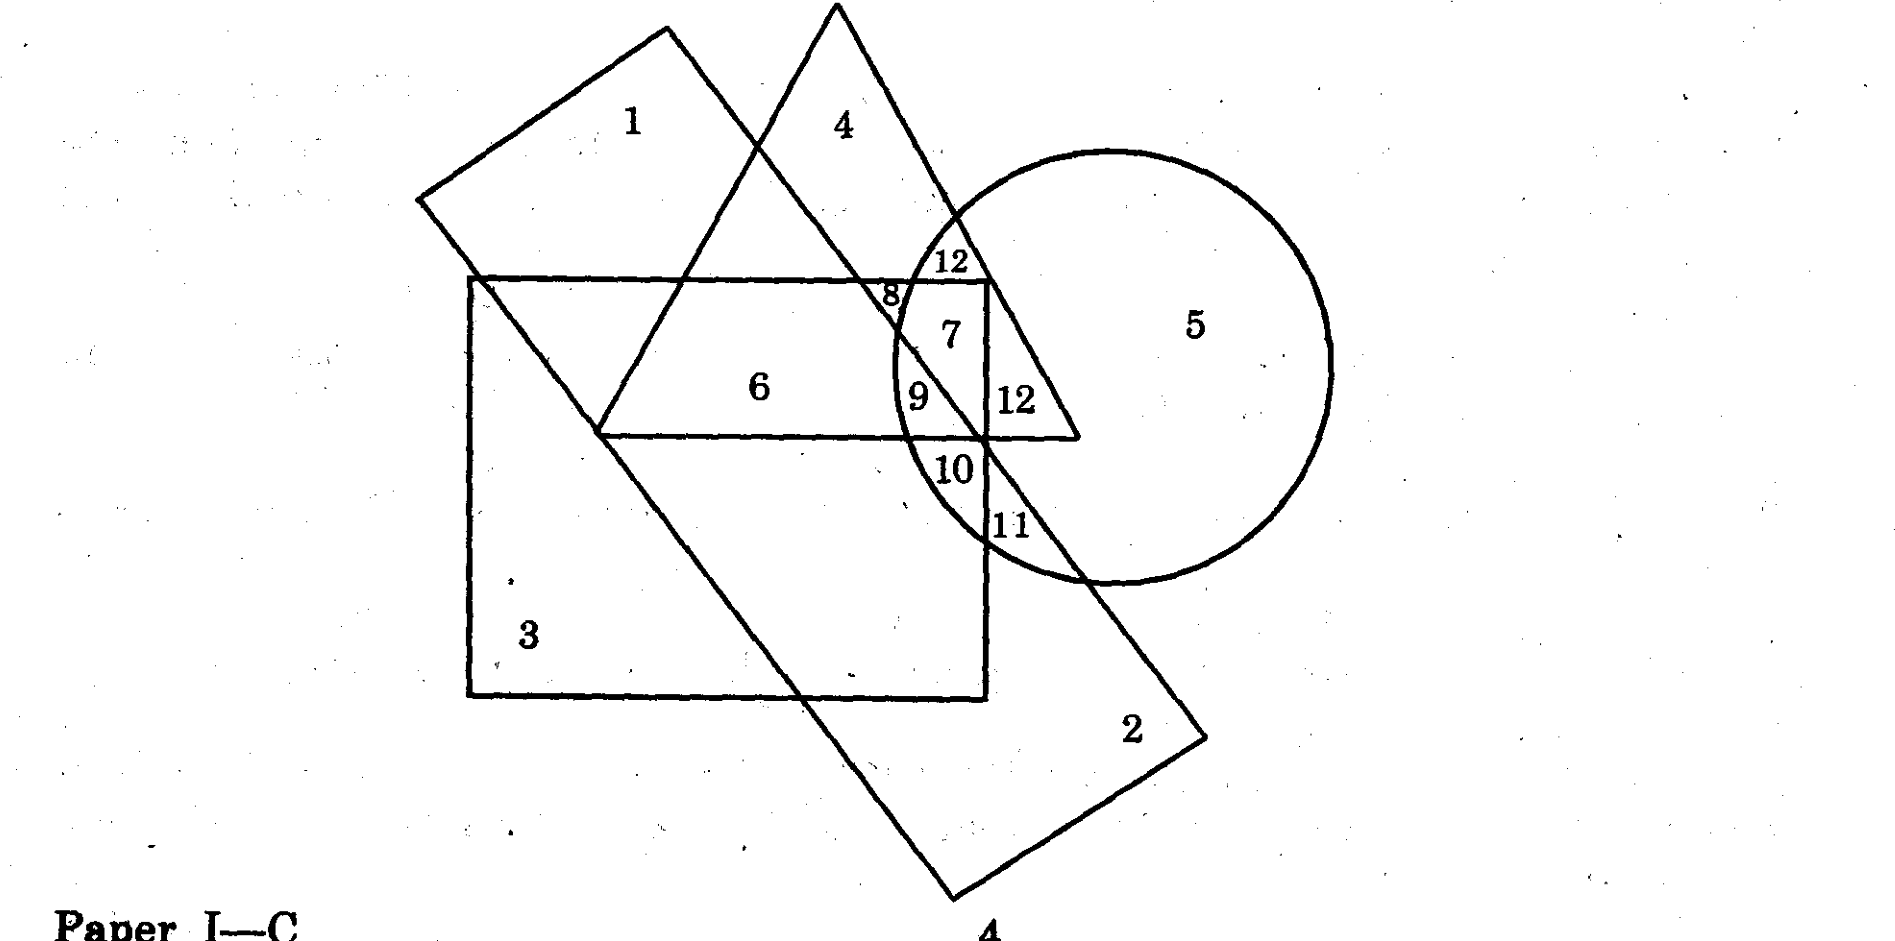
\includegraphics[width=0.72\linewidth]{fig/dec03_q6.png}\end{center}

%% Q6 q
Non-rural and hardworking medical students who are affluent are represented by the region:

%% Q6
Required: inside circle, square and tilted rectangle, but \textbf{outside the triangle}. That is region \textbf{10}.
\tip{Method for every such question: list the figures the region must be \emph{inside} and those it must be \emph{outside}, then find the single numbered region that satisfies all conditions.}

%% Q7
Inside circle and triangle; outside square and rectangle: region \textbf{12} (the part of the triangle inside the circle but above/right of the square and rectangle).

%% Q8
Inside circle, square and triangle; outside the rectangle: region \textbf{7}.

%% Q9
Inside the circle only (outside square, triangle and rectangle): region \textbf{5}.

%% Q10
Inside all four figures (circle, square, triangle, rectangle): region \textbf{9}.

%% Q11
Divide successively by 1, 2, 4, 8: $320\div1=320$, $\div2=160$, $\div4=40$, $\div8=\mathbf{5}$.

%% Q12
Each term $=$ previous $\times10-5$: $1\rightarrow5\rightarrow45\rightarrow445\rightarrow\mathbf{4445}$.

%% Q13
Each letter advances by 2: B$\rightarrow$D$\rightarrow$F$\rightarrow$\textbf{H}, H$\rightarrow$J$\rightarrow$L$\rightarrow$\textbf{N}, L$\rightarrow$N$\rightarrow$P$\rightarrow$\textbf{R}. Next: \textbf{HNR}.

%% Q14
First letters K, M, O, Q, \textbf{S} ($+2$); last letters Z, X, V, T, \textbf{R} ($-2$); middle letters U, O, I, E, \textbf{A} (moving back through the vowels). Next: \textbf{SAR}.

%% Q15
Filling c, a, b, c, a gives
\[\text{ab\underline{c}cba\underline{a}bcc\underline{b}aab\underline{c}cba\underline{a}b}=\text{abccba}\,|\,\text{abccba}\,|\,\text{abccba}\,|\,\text{ab}\]
The block ``abccba'' repeats, so the answer is \textbf{cabca}.

%% Q16
Filling the gaps with c, a, b, c, a, a (option A) completes the repeating letter pattern built from ``abc''. Answer as per key: \textbf{cabcaa}.

%% Q17
The cube is cut $5\times5\times5$. Let top and bottom be red, front and right green, left and back uncoloured.
On the front (green) face, remove the top row and bottom row (also red) and the column on the right edge (also green): $3\times4=12$ cubes have green only. Same for the right face.
Total $=12\times2=\mathbf{24}$.

%% Q18
Cubes with green on two faces lie along the common edge of the two green faces: $\mathbf{5}$ cubes (the two end cubes on this edge are also red, but they still carry green on two faces).

%% Q19 q
In the multiplication given below, find the digits corresponding to the letters:\\[3pt]
\centering\begin{tabular}{r} 6 b c\\ $\times$\ 3 5 d\\\hline 6 6 e\\ 3 3 3 0\ \ \\ 1 a a 8\ \ \ \ \\\hline 2 2 3 7 6 6\end{tabular}\\[3pt]
\raggedright `b' stands for:

%% Q19
The second partial product is $6bc\times5=3330$, so $6bc=666$. Hence \textbf{b $=$ 6} (and c $=6$, d $=1$, e $=6$, a $=9$: $666\times3=1998$).

%% Q20 q
In the same multiplication, `c' stands for:

%% Q20
From $6bc=666$ (because $6bc\times5=3330$): \textbf{c $=$ 6}.

%% Q21 ctx
\textbf{Q.~21--22:} A square cardboard ABCD, inside which the square JKLM is inscribed, is placed horizontally (and may be reversed). In each question, two conditions are given: (I) whether the cardboard is reversed; (II) the direction of one vertex with respect to the centre O. Find the direction of the other given vertex with respect to O.
\begin{center}
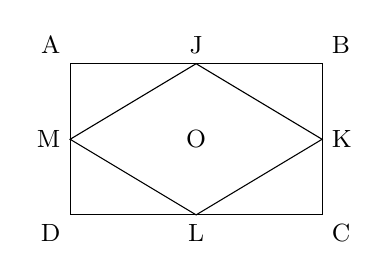
\begin{tikzpicture}[scale=0.8,font=\small]
\draw (0,0) rectangle (4,2.4); \draw (2,2.4)--(4,1.2)--(2,0)--(0,1.2)--cycle;
\node[above left] at (0,2.4){A}; \node[above right] at (4,2.4){B}; \node[below right] at (4,0){C}; \node[below left] at (0,0){D};
\node[above] at (2,2.4){J}; \node[right] at (4,1.2){K}; \node[below] at (2,0){L}; \node[left] at (0,1.2){M}; \node at (2,1.2){O};
\end{tikzpicture}
\end{center}
In the normal position: A $=$ NW, B $=$ NE, C $=$ SE, D $=$ SW; J $=$ N, K $=$ E, L $=$ S, M $=$ W.

%% Q21 q
(I) Not reversed. (II) A towards S. `J' will be in the direction:

%% Q21
A moves from NW to S: a rotation of $225^\circ$ clockwise (NW $\rightarrow$ N $\rightarrow$ \ldots\ $\rightarrow$ S is 5 steps of $45^\circ$). J (N) rotated $225^\circ$ clockwise points \textbf{SW}.

%% Q22 q
(I) Not reversed. (II) L towards NE. `M' will be in the direction:

%% Q22
L moves from S to NE: $225^\circ$ clockwise. M (W) rotated $225^\circ$ clockwise $\rightarrow$ \textbf{SE}.

%% Q23 note
By the given relations the daughter of I is IV. The official key gives (B) VI.

%% Q23
I is father of III and II is mother (III is son of II). III is brother of IV, and IV is \emph{not} son of I, so IV is I's \textbf{daughter}. V and VI are nephew and niece (children of a sibling). Logically the answer is IV; the key gives \textbf{VI}.

%% Q24
GOLD $\rightarrow$ EMJB: each letter moves 2 back. To decode NMPR, move each letter 2 forward: \textbf{PORT}.

%% Q25
The code replaces digit $n$ by the $n$-th letter: 6$\rightarrow$F, 7$\rightarrow$G, 4$\rightarrow$D, 3$\rightarrow$C. So 97285 $\rightarrow$ I G B H E $=$ \textbf{IGBHE}.

%% Q26 q
At a certain restaurant, above the kitchen door four small lights, numbered 1 to 4 from left to right, are used to signal waiters: I $=$ all four lights; II $=$ lights 1 and 2; III $=$ light 1 only; IV $=$ lights 2, 3 and 4; V $=$ lights 3 and 4. Not-working lights are taken as illuminated.\\ If lights two and three both are off, then the waiter signalled could be:

%% Q26
With lights 2 and 3 off, only signals that do not use 2 or 3 remain: III (light 1 only). \textbf{III}.

%% Q27 q
If lights one and two are not working (and hence count as illuminated), and lights three and four are illuminated, then the signal of which of the waiters (I, IV and V) might be signalled?

%% Q27
Lights 3 and 4 are on and lights 1 and 2 may or may not be intended, so the signal could be I (all four), IV (2, 3, 4) or V (3, 4): \textbf{I, IV and V}.

%% Q28 note
Strictly, steel (an alloy) is the odd one out among the metallic elements tin, iron and copper. The official key gives (D) Copper.

%% Q28
Tin, iron and copper are elements; steel is an alloy of iron. The official key, however, gives \textbf{Copper} (the only non-greyish, reddish metal of the group). Mark (D) as per the key.

%% Q29
Truthful, sly and virtuous describe a person's \emph{moral character}. \textbf{Pensive} (thoughtful) describes a \emph{mood}, so it is the odd one.

%% Q30
Required SP $=800\times1.125=900$. SP $=0.9\times$ MP, so MP $=900/0.9=$ \textbf{Rs.~1,000}.

%% Q31
Selective admission aims to \textbf{screen those who can benefit from higher education}, i.e.\ admit students with the required aptitude and preparation.

%% Q32
Per the key, the least helpful step is option (D), discussing the plan with others. Deciding content, choosing methodology and knowing the students' background are essential parts of lecture planning.

%% Q33
Interactive sessions \textbf{enhance students' involvement}, which improves understanding and retention.

%% Q34
NAAC evaluation helps an institution \textbf{know its strengths and weaknesses}, so that it can improve quality.

%% Q35
Adolescents are strongly influenced by their peer group, so \textbf{peer and compeer approval} is the most powerful incentive.

%% Q36
A Chief Proctor's office is justified because \textbf{students' activities and programmes need regulatory control} (discipline and order on campus).

%% Q37
\textbf{Action research} focuses on improving one's own work situation or practice.

%% Q38
Sampling is economical, saves time, and (because a smaller group can be studied more carefully) can improve accuracy: \textbf{all the above}.

%% Q39
Frequency counts in a $2\times3$ contingency table call for the \textbf{chi-square test}, a non-parametric test.

%% Q40
The main purpose of reporting research is to \textbf{highlight the factual position}, i.e.\ to present the findings honestly and objectively.

%% Q41
\textbf{Abdicate} means to give up (a throne or responsibility), i.e.\ \textbf{renounce}.

%% Q42
\textbf{Sham} means something false or fake, i.e.\ \textbf{pretence}.

%% Q43
The research method combines \textbf{inductive and deductive reasoning} (the reflective or scientific method).

%% Q44
Feedback is the response that comes back to information. Similarly, reaction is the response to \textbf{action}.

%% Q45
Per the official key, the pair is \textbf{Deaden : Diffuse}, i.e.\ the second word is the (intensified) result of the first, as detonation follows activation.

%% Q46 ctx
\textbf{Q.~46--50:} Read the passage given below and answer the questions.\par\smallskip
Competition the world over is slowly becoming a lethal agent in killing the regenerative process among human beings. This is happening through a vicious cycle of anxiety--tension--stress--depression--nervous breakdown. The problem percolates to the entire human structure touching health of the body, mind and spirit. To prepare a sound mind in a sound body is a coveted definition of education. But in the present life-cycle dynamics everything seems to explode. More so for those aspiring to be competitive winners irrespective of the field, the killer instinct is soon becoming a self killing process. Much has been spoken and written about the evil effects of stress and its psychosomatic repercussions. Many solutions have been offered by counselling agencies across the globe --- some bordering on spiritual remedies, while large chunk depending upon psychiatric-psychic process. Many have also recommended physical activity to control stress and depression. However, an integrated approach to life management programme in the competitive environment could probably be the most easy and efficient course of remedy. But what is not clearly taken into reckoning is the fact that the body, the mind and the spirit all the three together form an individual and therefore, the health of each of these three components is equally important and has a separate existence. For instance, when the mind is disturbed, thereby creating unhealthiness in the intellectual-emotional plane, the body despite being in absolute physical comfort still gets affected and is often the victim. Therefore, it is necessary to understand fear and conquer it at the first place in order to arrest spread of anxiety, stress, tension and depression.

%% Q46 q
Basic objective of this passage is to project:

%% Q46
The passage traces how competition produces anxiety, stress and depression and affects body, mind and spirit, i.e.\ the \textbf{causes of mental ill health}.

%% Q47 q
After going through this passage, two premises come up. You are to indicate which is right.\\
I. Anxiety leads to nervous breakdown.\\ II. Stress has evil effects on health.

%% Q47
Per the key, only II is right: the passage directly states the ``evil effects of stress and its psychosomatic repercussions''. Anxiety is only the first link of a cycle, not directly said to cause breakdown.

%% Q48
The passage explains a problem, its causes and possible remedies, so it is \textbf{explanatory}.

%% Q49
The passage ends with the need to understand fear and arrest stress, anxiety and depression, so the best title is \textbf{Overcoming Stress}.

%% Q50
A ``disturbed mind'' is an \textbf{agitated mind}.
